\documentclass[number]{ximera}

%\usepackage{tikz}

\renewcommand{\theenumi}{\arabic{enumi}.}


% set font encoding for PDFLaTeX, XeLaTeX, or LuaTeX
\usepackage{ifxetex,ifluatex}
\newif\ifxetexorluatex
\ifxetex
  \xetexorluatextrue
\else
  \ifluatex
    \xetexorluatextrue
  \else
    \xetexorluatexfalse
  \fi
\fi

\ifxetexorluatex
  \usepackage{fontspec}
\else
  \usepackage[T1]{fontenc}
  \usepackage[utf8]{inputenc}
  \usepackage{lmodern}
\fi

\usepackage{hyperref}
\usepackage{tikz} %% Adding this here so it's not manually added elsewhere

%My github password is ximera1
%My GeoGebra password is Ximera1

\title{Special Triangles}
\author{Univ. of Minnesota MathCEP}

\begin{document}

\begin{abstract}
Recall that a triangle has three angles that add up to $180^\circ$.
A right triangle is a triangle that has one $90^\circ$ angle; the side opposite this angle is called the hypotenuse.
In this activity, we will look at two special cases of right triangles: when the remaining two angles are each $45^\circ$, and when the remaining two angles are $30^\circ$ and $60^\circ$.
Our goal is to determine the lengths of the legs of these triangles when the hypotenuse is 1.
\end{abstract}

\maketitle

For the $45^\circ-45^\circ-90^\circ$ triangle, (the isosceles right triangle), there are two legs of length $a$
and the hypotenuse of length 1.

\begin{figure}[h!]
\begin{tikzpicture}[scale=2]
		\draw (0,0) -- node[below] {$a$} (2,0) -- node[above right] {$1$} (0,2) -- node[left] {$a$} (0,0) -- cycle;
		\draw (0,0.2) -- (0.2,0.2) -- (0.2,0);
		\node at (1.6,0.15) {$45^\circ$};	
		\node at (0.2,1.55) {$45^\circ$};	
\end{tikzpicture}			
\caption{A $45^\circ-45^\circ-90^\circ$ triangle.}
\end{figure}


\begin{problem}
Use the Pythagorean Theorem to write an equation relating the lengths of the sides of the triangle: $\answer{a}^2+\answer{a}^2=\answer{1}^2$.
\begin{hint}
In a right triangle with sides lengths $a$ and $b$ and hypotenuse $c$, the Pythagorean Theorem states that $a^2+b^2=c^2$.
\end{hint}

\end{problem}

\begin{problem}
Solve the equation for $a = \answer{\frac{\sqrt{2}}{2}}$.
\end{problem}

To find the lengths of the legs of the $30^\circ-60^\circ-90^\circ$ triangle, begin with an equilateral triangle, all of whose sides are length 1.

\begin{figure}[h!]
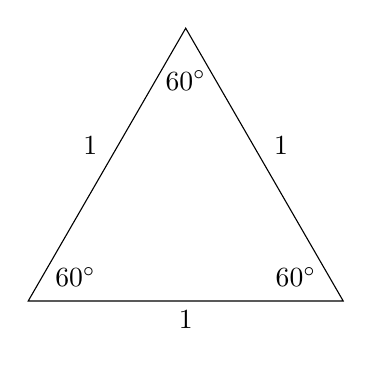
\begin{tikzpicture}[scale=2]
		\draw (0,0) -- node[below] {$1$} (2,0) -- node[above right] {$1$} (1,1.732) -- node[above left] {$1$} (0,0) -- cycle;
		\node at (0.3,0.15) {$60^\circ$};		
		\node at (1,1.4) {$60^\circ$};		
		\node at (1.7,0.15) {$60^\circ$};		
\end{tikzpicture}			
\caption{An equilateral triangle.}
\end{figure}



\begin{problem}
Solve for the height $h$ of the 30-60-90 triangle. One possible approach is the following:

\begin{itemize}
\item From the top vertex, draw a line segment perpendicular to the bottom side, cutting the original triangle into two congruent triangles. 
\begin{hint}
In an equilateral triangle, this line segment is called a perpendicuar bisector, a median, and an altitude.
\end{hint}
\item Find the lengths of the two halves of the bottom side.
\item Find all the angles in the triangles.
\item Label the length of the altitude $h$.
\item Use the Pythagorean Theorem to write an equation involving $h$:
\[\answer{h}^2 + \answer{\frac{1}{2}}^2 = \answer{1}^2\]
\item Solve the equation for $h = \answer{\frac{\sqrt{3}}{2}}$.
\end{itemize}
\end{problem}

\begin{problem} Draw the 45-45-90 triangle in as many orientations as possible, keeping the legs either horizontal or vertical. How many are there? $\answer{4}$
\begin{hint}
You can rotate and reflect the triangle.
\end{hint}
\end{problem}

\begin{problem} Draw the 30-60-90 triangle in as many orientations as possible, keeping the legs either horizontal or vertical. How many are there? $\answer{8}$
\begin{hint}
Do you expect this number to be the same as in the 45-45-90 case?
\end{hint}

\end{problem}




\end{document}

